\chapter{Fundamental solutions in Minkowski spacetime}
\label{chapter2}

In this chapter, we illustrate the concept of fundamental solutions and their use in solving initial value problems. We focus on the case of the d'Alembert wave operator $\Box$ built on top of the $n$-dimensional Minkowski spacetime $\mathbb{M}^n$.\\
Two different approaches will be followed. The first relies on the Fourier transform. It is useful to build explicit formulas for the fundamental solutions in the lower dimensional cases and to show the existence of such solutions in the general case.
The second approach, via Riesz distributions, is useful for its generality and because it will be used in the next chapter to construct fundamental solutions on suitable Lorentzian manifolds, although it is more abstract and does not lead to explicit formulas.\\
We will find two independent fundamental solutions, the \emph{retarded} and the \emph{advanced} one, that preserve the causal structure of the spacetime, i.e. that propagate the source of the equation respectively in the causal future and in the causal past, in accordance with the causality principle.\\


\section{Fundamental solutions}
\begin{definition}
	Let $P$ be a differential operator on a manifold $\mM$ and $x_0\in\mM$. A \textbf{fundamental solution} for $P$ at $x_0$ is a distribution $u_{x_0}\in\mD'(\mM)$ such that
	\[Pu_{x_0}=\delta_{x_0},\]
	where $\delta_{x_0}$ is the Dirac delta distribution in $x_0$, i.e. $(\delta_{x_0},f)=f(x_0)$ for all $f\in\mD(\mM)$.
\end{definition}

\noindent Following the previous definition\footnote{see [\citealp[Ch. 2]{bar2}] and [\citealp{ginoux}]}, assume that a fundamental solution $u_x$ $u_x$ has a continuous dependence on $x$ (i.e. the function $x\mapsto(u_x,\varphi)$ is continuous for all $\varphi\in\mD(\mM)$) and $\psi\in\mD(\mM)$, then $F_\psi:=(u_x,\psi)$ is a solution for the differential equation
	\[	PF_\psi=\psi.		\]
	This comes applying the operator $P$ on $F_\psi$, for which one obtains
	\[	PF_\psi=(u_x,P^*\psi)=(Pu_x,\psi)=(\delta_{x},\psi)=\psi(x),		\]where $P^*$ stands for the formal adjoint of $P$.


\section{The d'Alembert wave operator in Minkowski}
In order to be more concrete, we begin by computing the fundamental solution of $\Box$ in $\mathbb{M}^n$ with $2\leq n\leq 4$.\\
As we recalled in the previous chapter, the d'Alembert wave operator is defined in $\mathbb{M}^n$, with respect to the variables $x=(t,\mathbf{x})$, as $$\ds\Box:=\frac{\partial^2}{\partial t^2}-\sum_{i=1}^{n-1}\frac{\partial^2}{\partial x_i^2}=-\partial^i\partial_i.$$
We will find two fundamental solutions $G_{x_0}^+,G_{x_0}^-\in\mD'(\mathbb{M}^n)$ for $\Box$ at $x_0\in \mathbb{M}^n$ with the following properties
\begin{equation}
	\supp(G_{x_0}^+)	\subset J_+(x_0),\qquad \supp(G_{x_0}^-)	\subset J_-(x_0).
	\label{eq:supporti}
\end{equation}
Such solutions will be called respectively \textbf{retarded} ($G_+$) and \textbf{advanced} ($G_-$) fundamental solutions.\\
In order to find the fundamental solutions at $x_0$, the following proposition guarantees it suffices to solve the problem $\Box u_0=\delta_0$.
\begin{prop}
	Let $x_0\in\mathbb{M}^n$ and $T_{x_0}$ be the translation operator as in Definition \ref{defn:transl}. Then $[\Box,T_{x_0}]=0$ (i.e. $\Box$ and $T_{x_0}$ commute) and a fundamental solution for $\Box$ at $x_0$ is
	\[	u_{x_0}=T_{x_0}u_0,	\]	
	where $u_0$ is a fundamental solution at $0$.
\end{prop}
	
\Proof Let $\varphi\in\mD(\mathbb{M}^n)$, then
\[	\left(\Box T_{x_0}u,\varphi(x)\right)=\left( T_{x_0}u,\Box\varphi(x)\right)=\left( u,\Box\varphi(x+x_0)\right)=	\]
\[	=\left(\Box u,\varphi(x+x_0)\right)=\left(T_{x_0}\Box u,\varphi(x)\right),	\]where it was used the fact that $\Box$ is formally self-adjoint and invariant under translations when acting on smooth functions. 
Hence, it holds
\[\Box\left(T_{x_0}u_0\right)=	T_{x_0}\left(\Box u_0\right)=T_{x_0}\delta_0=\delta_{x_0},	\]
because $\Box$ and $T_{x_0}$ commute, so $T_{x_0}u_0$ is a fundamental solution at $x_0$.  \endproof\\

\begin{prop}
	Let $\psi\in\mD(\mathbb{M}^n)$. Then
	\begin{equation}
		F_\psi=u_0*\psi\in C^\infty(\mathbb{M}^n)
	\end{equation}
	is a (smooth) solution for the differential equation
	$	PF_\psi=\psi$ (here $*$ denotes convolution).
	\label{prop:regularity}
\end{prop}
\Proof Since $u_x=T_xu_0$ and $F_\psi=(u_x,\psi)=(T_xu_0,\psi)$ is a solution to the equation, the thesis follows immediately noting that, by definition, $(T_xu_0,\psi)=(u_0*\psi)(x)$. The smoothness of the solution follows from Theorem \ref{th:convolutionregularity}.\endproof

\section{The Fourier transform approach}
In order to employ the theory of Fourier transforms, it is necessary to work with distributions in $\mathcal{S}'(\mathbb{M}^n)$.\\
We shall begin with a lemma that helps in the computations:
\begin{lem}
	For $u\in\mathcal{S}'(\mathbb{M}^n)$ if we let $x=(t,\mathbf{x})=(t,x_1,\dots,x_{n-1})$ and $k=(\omega,\mathbf{k})=(\omega,k_1,\dots,k_{n-1})$, it holds
	\begin{equation}
	\widehat{\Box\, u}(k)=\norm{k}^2\hat{u}=(|\mathbf{k}|^2-\omega^2)\hat{u}(k).
	\end{equation}
\end{lem}
\Proof For any test function $f\in\mathcal{S}(\mathbb{M}^n)$, and for any $u\in\mathcal{S}'(\mathbb{M}^n)$ $(\Box u,f)=(u,\Box f)$. Note that $$\Box_x\widehat{f}(k)=\int_{\mR^n}\Box_x f(x) e^{-i\langle k,x\rangle_0}\,\dd x=$$
$$=\int_{\mR^n}f(x)\,(|\mathbf{k}|^2-\omega^2)e^{-i\langle k,x\rangle_0}\,\dd x=(|\mathbf{k}|^2-\omega^2)\widehat{f}(k)$$ from which it descends
\[	(\widehat{\Box u},f)=(\Box u,\widehat{f})=(u,\Box\widehat{f})=(|\mathbf{k}|^2-\omega^2)(\widehat{u},f).		\]\endproof


\noindent Following [\citealp[Ch. 5]{jonsson}], we start by transforming the equation:
\begin{equation}	\widehat{\Box u}(k)=\hat{\delta}(k) \Rightarrow	(|\mathbf{k}|^2-\omega^2)\hat{u}(k)=1
\label{eq:fourierequation}
\end{equation}	

\noindent The difference of two solutions $\hat{u}\in\mathcal{S}'(\mathbb{M}^n)$, is a solution $\hat{v}$ to the equation
\begin{equation}
	(|\mathbf{k}|^2-\omega^2)\hat{v}(k)=0.
	\label{eq:homogeneous}
\end{equation}
This equation can be seen as the Fourier transform of the correspondent homogeneous equation $\Box v=0$. Hence $\widehat{u}+\widehat{v}$ is the transform of the sum of a particular solution for $\Box$ and a solution of the homogeneous equation, then it is a solution for Equation \eqref{eq:fourierequation}.\\

\noindent If we concentrate on the solutions for Equation \eqref{eq:homogeneous}, it is easy to see with a direct computation that any distribution of the form $$\hat{v}(k)=A(k)\delta(|\mathbf{k}|^2-\omega^2),$$ where $A(k)$ is any suitably regular function of $k$, solves the equation, because the Dirac delta is supported on $\{k\in\mR^n\,|\,|\mathbf{k}|^2-\omega^2=0\}$. Any solution to the homogeneous wave equation can be obtained by the inverse transform of $\widehat{v}$:
\[	v(x)=(2\pi)^{-n}	\int_{\mR^n} e^{i\langle k,x\rangle_0}A(k)\delta(|\mathbf{k}|^2-\omega^2)\,\dd k.	\]
Making use of formula (\ref{eq:delta1}), the last expression becomes
\begin{equation}
\begin{split}
v(x)=(2\pi)^{-n}	\int_{\mR^n} e^{i\langle k,x\rangle_0}\frac{A(k)}{2|\mathbf{k}|}\left[\delta(|\mathbf{k}|-\omega)+\delta(|\mathbf{k}|+\omega)\right]\,\dd k=\\
=(2\pi)^{-n}	\int_{\mR^{n-1}}\dd\mathbf{k}\,e^{i\mathbf{k}\cdot\mathbf{x}}\frac{e^{i|\mf{k}|t}A(k)|_{|\mf{k}|=\omega}+e^{-i|\mf{k}|t}A(k)|_{|\mf{k}|=-\omega}}{|\mf{k}|}.\end{split}
\label{eq:homo}
\end{equation}	



To solve for $\widehat{u}$ it is tempting to write
\[	\hat{u}(k)=\frac{1}{|\mathbf{k}|^2-\omega^2}=\frac{1}{(|\mathbf{k}|-\omega)(|\mathbf{k}|+\omega)},%+A(k)\delta(|\mathbf{k}|^2-\omega^2),
\]
which is ill-defined as a distribution wherever $\langle k,k\rangle_0=0$, i.e. on the light-cone of the Fourier space. Hence, we will define $\hat{u}$ as limit of a sequence of distributions depending on the parameter $\epsilon$
\[	\hat{u}_\epsilon=\frac{1}{|\mathbf{k}|^2-(\omega\pm i\epsilon)^2}=\frac{1}{(|\mathbf{k}|\mp i\epsilon-\omega)(|\mathbf{k}|\pm i\epsilon+\omega)}		\]
promoting $\omega$ to a complex variable and taking the limit for $\epsilon\to 0^+$ after performing the inverse transform. The choice of the signs in such expressions leads to different fundamental solutions.
\section{Fundamental solutions via Fourier transform}
\label{sec:fundafourier}
	The distributions $G_+$ and $G_-$ in $\mathcal{S}'(\mathbb{M}^n)$, defined respectively as the weak limit for $\epsilon\to 0^+$ of
	\begin{equation}
	G_\epsilon^+(x)=\frac{1}{(2\pi)^n}\int_{\mR^n}\frac{e^{i\langle k,x\rangle_0}}{|\mathbf{k}|^2-(\omega+ i\epsilon)^2}\,\dd k,
	\label{eq:retardedfourier}
	\end{equation}
	\begin{equation}
	G_\epsilon^-(x)=\frac{1}{(2\pi)^n}\int_{\mR^n}\frac{e^{i\langle k,x\rangle_0}}{|\mathbf{k}|^2-(\omega- i\epsilon)^2}\,\dd k,
	\label{eq:advancedfourier}
	\end{equation}	
are respectively a \textbf{retarded} and an \textbf{advanced} fundamental solutions at $x_0=0$ for the d'Alembert wave operator.\\
The aim is to prove that $\supp(G_+)	\subset J_+(0)$ and $\supp(G_-)	\subset J_-(0)$, and we proceed firstly by calculating the explicit formula for $2\leq n\leq 4$ and then discuss the general case via Riesz distributions.\\

%\noindent We will show that, if we denote with $d:=n-1$ the spatial dimensions, the retarded fundamental solutions $G_{(d)}^+$ turn out to be 
%\[G_{(1)}^{+}(t,x)=\frac{\Theta(t-|x|)}{2},\quad G_{(2)}^{+}(t,\mf{x})=\frac{\Theta( t)}{2\pi}\frac{\Theta(t^2-|\mf{x}|^2)}{\sqrt{t^2-|\mf{x}|^2}},\]

%\[G_{(3)}^{+}(t,\mf{x})=\frac{\Theta( t)}{4\pi}\frac{\delta(t- |\mf{x}|)}{|\mf{x}|}.\]


\noindent We compute $G_\pm$ as a limit of the inverse of the Fourier transform:
\[		G_\epsilon^{\pm}(x)=(2\pi)^{-n}\int_{\mR^n}\frac{e^{i\langle k,x\rangle_0}}{|\mathbf{k}|^2-(\omega\pm i\epsilon)^2}\,\dd k\]
%\[+(2\pi)^{-n}\left(A(k)\delta(|\mathbf{k}|^2-\omega^2),e^{i\langle k,x\rangle_0}\right)=\]
\begin{equation}=(2\pi)^{-n}	\int_{\mR^{n-1}}\dd\mathbf{k}\,e^{i\mathbf{k}\cdot\mathbf{x}}\int_{-\infty}^{+\infty}\frac{e^{-i\omega t}}{|\mathbf{k}|^2-(\omega\pm i\epsilon)^2}\,\dd\omega. \label{eq:fourierinverse}	\end{equation}


\subsection*{Computing the complex integrals}
In order to calculate the inner integral in the former expression,

\[\tilde{G}_\epsilon^{\pm}(t,\mathbf{k}):=\int_{-\infty}^{+\infty}\frac{e^{-i\omega t}}{|\mathbf{k}|^2-(\omega\pm i\epsilon)^2}\,\dd\omega,\]

we make use of techniques of complex analysis as follows.\\
\begin{figure}[h]
	\centering
	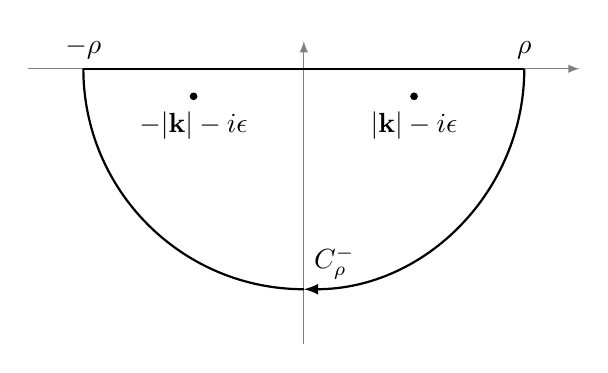
\begin{tikzpicture}[scale=0.7][>=latex]
	\coordinate (Origin)   at (0,0);
	\coordinate (XAxisMin) at (-5,0);
	\coordinate (XAxisMax) at (5,0);
	\coordinate (YAxisMin) at (0,-5);
	\coordinate (YAxisMax) at (0,0.5);
	\draw [thin, gray,-latex] (XAxisMin) -- (XAxisMax) ;% Draw x axis
	\draw [thin, gray,-latex] (YAxisMin) -- (YAxisMax) ;% Draw y axis
	
	%\clip (-5,-5) rectangle (10cm,10cm); % Clips the picture...
	
	
	
	\draw [thick,-latex] (4cm,0mm) node[above] {$\rho$} arc [start angle=0, end angle=-90, radius=4cm] node[above right] {$C_\rho^-$};
	\draw [thick] (0,-4cm) arc [start angle=-90, end angle=-180, radius=4cm] node[above] {$-\rho$};
	\draw [thick] (-4,0) -- (4,0);
	
	\draw (-2,-0.6) node[below] {$-|\mathbf{k|}-i\epsilon$};
	\draw (2,-0.6) node[below] {$|\mathbf{k|}-i\epsilon$};
	\fill (-2,-0.5) circle (0.07);
	\fill (2,-0.5) circle (0.07);
	
	
	
	
	
	
	\end{tikzpicture}

	\caption{The circuit to compute $\tilde{G}_\epsilon^{+}(t,\mathbf{k})$ for $t>0$.}	\label{fig:integrale2}
	
\end{figure}
Denote
\begin{itemize}
	\item $C_\rho^+$ the upper half-circle of radius $\rho$ centered at $\omega=0$ which has $\Im(\omega)>0$, oriented counter-clockwise;
	\item $C_\rho^-$ the lower half-circle of radius $\rho$ centered at $\omega=0$ which has $\Im(\omega)<0$, oriented clockwise;
	\item $[-\rho,\rho]$ the interval of the real line connecting $-\rho$ and $\rho$, oriented from left to right.
\end{itemize}
\begin{figure}[h]
	\centering
	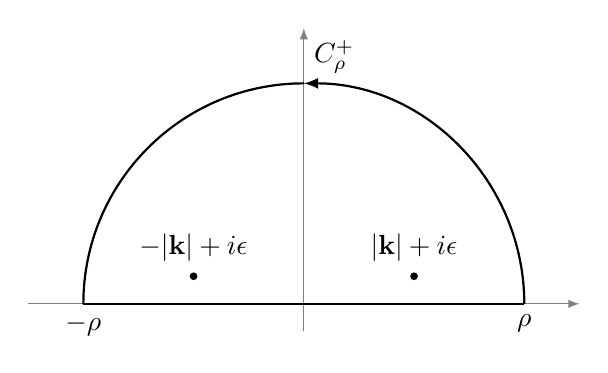
\begin{tikzpicture}[scale=0.7][>=latex]
	\coordinate (Origin)   at (0,0);
	\coordinate (XAxisMin) at (-5,0);
	\coordinate (XAxisMax) at (5,0);
	\coordinate (YAxisMin) at (0,-0.5);
	\coordinate (YAxisMax) at (0,5);
	\draw [thin, gray,-latex] (XAxisMin) -- (XAxisMax) ;% Draw x axis
	\draw [thin, gray,-latex] (YAxisMin) -- (YAxisMax) ;% Draw y axis
	
	%\clip (-5,-5) rectangle (10cm,10cm); % Clips the picture...
	
	
	
	\draw [thick,-latex] (4cm,0mm) node[below] {$\rho$} arc [start angle=0, end angle=90, radius=4cm] node[above right] {$C_\rho^+$};
	\draw [thick] (0,4cm) arc [start angle=90, end angle=180, radius=4cm] node[below] {$-\rho$};
	\draw [thick] (-4,0) -- (4,0);
	
	\draw (-2,0.6) node[above] {$-|\mathbf{k|}+i\epsilon$};
	\draw (2,0.6) node[above] {$|\mathbf{k|}+i\epsilon$};
	\fill (-2,0.5) circle (0.07);
	\fill (2,0.5) circle (0.07);
	
	
	
	
	
	
	\end{tikzpicture}

	\caption{The circuit to compute $\tilde{G}_\epsilon^{-}(t,\mathbf{k})$ for $t<0$.}
	\label{fig:integrale1}
\end{figure}

The singularities are
\[\text{for } \tilde{G}_\epsilon^{+}:\quad \omega=\pm|\mathbf{k}|-i\epsilon,\]
\[\text{for } \tilde{G}_\epsilon^{-}:\quad \omega=\pm|\mathbf{k}|+i\epsilon.\]
Hence we have
\[\text{for } t<0\quad  \tilde{G}_\epsilon^{+}(t,\mathbf{k})=\lim_{\rho\to\infty}\int_{C_\rho^++[-\rho,\rho]}\frac{e^{-i\omega t}}{|\mathbf{k}|^2-(\omega+ i\epsilon)^2}\,\dd\omega=2\pi i\sum\operatorname{Res}=0,\]
where the sum is extended to the singularities in the upper half-plane. The expression vanishes because we choose the circuit such that the integral on $C_\rho^+$ vanishes in virtue of Jordan's lemma and there are no singularities in the region bounded by the circuit.\\
For the same reasons
\[\text{for } t>0,\  \tilde{G}_\epsilon^{-}(t,\mathbf{k})=\lim_{\rho\to\infty}\int_{C_\rho^-+[-\rho,\rho]}\frac{e^{-i\omega t}}{|\mathbf{k}|^2-(\omega- i\epsilon)^2}\,\dd\omega=-2\pi i\sum\operatorname{Res}=0,\]
where the sum is extended th the singularities of the function in the lower half-plane and the minus sign arises because of the clockwise circuit.\\
The non-zero integrals are
\[	\tilde{G}_\epsilon^{+}(t,\mathbf{k}), \text{ for } t>0,\qquad \tilde{G}_\epsilon^{-}(t,\mathbf{k}),\text{ for } t<0.	\] 
The first is computed via the lower circuit in \textsc{Figure} (\ref{fig:integrale2}): $C_\rho^-+[-\rho,\rho]$, the second via the upper counterpart in \textsc{Figure} (\ref{fig:integrale1}): $C_\rho^++[-\rho,\rho]$, in order to get rid of contributes from the half-circles.\\

The results are 
\[	\text{for } t>0\quad \tilde{G}_\epsilon^{+}(t,\mathbf{k})=2\pi ie^{-\epsilon|\mf{k}| t}\left(\frac{e^{-i|\mathbf{k}|t}-e^{i|\mathbf{k}|t}}{2|\mathbf{k}|}\right)=2\pi \frac{\sin|\mathbf{k}|t}{|\mathbf{k}|}e^{-\epsilon|\mf{k}| t},		\]
\[	\text{for } t<0\quad \tilde{G}_\epsilon^{-}(t,\mathbf{k})=-2\pi ie^{\epsilon|\mf{k}| t}\left(\frac{e^{-i|\mathbf{k}|t}-e^{i|\mathbf{k}|t}}{2|\mathbf{k}|}\right)=-2\pi \frac{\sin|\mathbf{k}|t}{|\mathbf{k}|}e^{\epsilon|\mf{k}| t}.		\]
Summing up everything in one formula:
\begin{equation}
	\tilde{G}_\epsilon^{\pm}(t,\mathbf{k})=\pm 2\pi\Theta(\pm t)\frac{\sin|\mathbf{k}|t}{|\mathbf{k}|}e^{\mp\epsilon|\mf{k}| t},
	\label{eq:integralone}
\end{equation}
where $\Theta$ is the Heaviside step-function.\\
It can be noticed that
\[	\tilde{G}_\epsilon^{+}(t,\mathbf{k})=\tilde{G}_\epsilon^{-}(-t,\mf{k}),		\]
because of the parity of sine function. So, we can deduce that the \textbf{advanced} solution can be calculated from the retarded one via time inversion:
\begin{equation}
	G_-(t,\mf{x})=G_+(-t,\mf{x}).
\end{equation}

\noindent We can now show that the support $G_\pm$ is included in $J_+(0)\cup J_-(0)$.
\begin{prop}
	If $x\in\mathbb{M}^n$ satisfies $\gamma(x)<0$ (where $\gamma$ is defined in Definition \ref{defn:gamma}), $G_\pm(x)=0$.
	\label{prop:spacelike}
\end{prop}
\Proof Consider a reference frame $R$ in which $x=(t,\mf{x})$ and suppose for now $t\geq 0$. It descends $G_+(x)=0$.  Since $G_\pm$ are manifestly Lorentz invariant and $\gamma(x)<0$, one can find a reference frame $R'$ in which $x=(t',\mf{x}')$ and $t'<0$, so that $G_-(x)=0$. The converse can be treated similarly. \endproof\\

\noindent We can focus once more on equation (\ref{eq:fourierinverse}) to show explicit solutions for spatial dimensions $d$ ranging from $1$ to $3$:
\begin{equation*}
	G_{(d)}^{+}(x)=\frac1{(2\pi)^{d+1}}\lim_{\epsilon\to 0^+}\int_{\mR^{d}}\dd\mathbf{k}\,e^{i\mathbf{k}\cdot\mathbf{x}}\tilde{G}_\epsilon^{+}(t,\mathbf{k})=\end{equation*} 
	\begin{equation*}
	=\lim_{\epsilon\to 0^+}\frac{\Theta(t)}{(2\pi)^{d}}\int_{\mR^{d}}\dd\mathbf{k}\,e^{i\mathbf{k}\cdot\mathbf{x}}\, \frac{\sin|\mathbf{k}|t}{|\mathbf{k}|}e^{-\epsilon|\mf{k}| t}.
\end{equation*}

\subsection*{Dimension $n=1+1$ - wave on a line}
The integral we have to make is:

\begin{figure}[h]
	\centering
	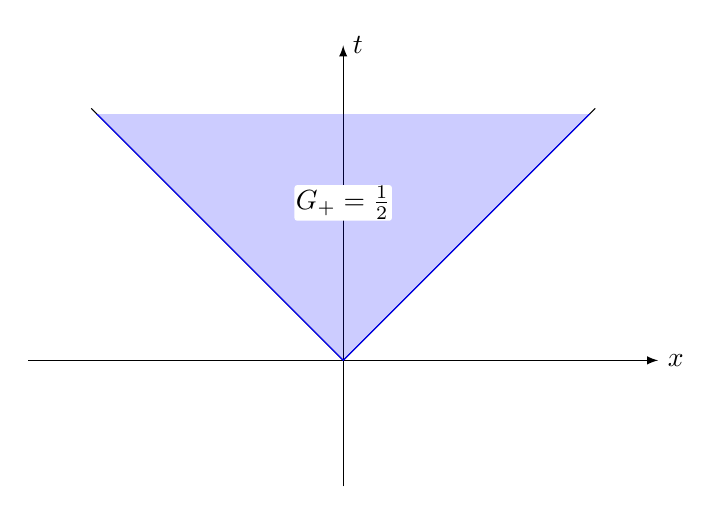
\begin{tikzpicture}[scale=0.8][>=latex]
	\coordinate (Origin)   at (0,0);
	\coordinate (XAxisMin) at (-5,0);
	\coordinate (XAxisMax) at (5,0);
	\coordinate (YAxisMin) at (0,-2);
	\coordinate (YAxisMax) at (0,5);
	\draw [thin,-latex] (XAxisMin) -- (XAxisMax) node[right] {$x$};% Draw x axis
	\draw [thin,-latex] (YAxisMin) -- (YAxisMax) node[right] {$t$};% Draw y axis
	
	%\clip (-5,-5) rectangle (10cm,10cm); % Clips the picture...
	
	\draw[thin] (0,0) -- (4,4);
	\draw[thin] (0,0) -- (-4,4);
	\begin{scope}
	\clip (-4,0) -- (4,0) -- (4,3.9)-- (-4,3.9) --cycle;
	\draw [thin, color=blue, fill=blue, fill opacity=0.2] (0,0) -- (4,4) -- (-4,4) --cycle ;
	\end{scope}
	\node[fill=white,rounded corners=1pt,inner sep=0.5pt] at (0,2.5) {$G_+=\frac{1}{2}$};
	
	
	
	
	
	
	\end{tikzpicture}

	\caption{The support of $G_+$ in 1+1 dimensional case.}
		\label{fig:1Dretarded}
\end{figure}
\begin{equation*}
G_{(1)}^{+}(t,x)=\frac{\Theta( t)}{2\pi}\lim_{\epsilon\to 0^+}\int_{-\infty}^{+\infty}\dd k\,e^{ik\cdot x}\, \frac{\sin kt}{k}e^{-\epsilon k t}.
\end{equation*}
It holds $$\int_{-\infty}^{+\infty}\dd k\,e^{ik\cdot (x+i\epsilon t)}\, \frac{\sin kt}{k}\mathop{=}^{k\rightarrow k'=kt}\int_{-\infty}^{+\infty}\dd k\,e^{ik\cdot (x/t+i\epsilon )}\, \frac{\sin k}{k}\mathop{\longrightarrow}_{\epsilon\to 0^+}$$ $$\longrightarrow\pi {\chi}_{[-1,1]}\left(\frac{x}{t}\right)=\pi\chi_{[-t,t]}(x),$$
where
\[	\chi_{[a,b]}(z)=\begin{cases} 1, & \mbox{if } z\in[a,b] \\ 0, & \mbox{otherwise, }
\end{cases}		\]
Finally the integrals become
\begin{equation*}
G_{(1)}^{+}(t,x)=\frac{\Theta( t)}{2}\chi_{[-t,t]}(x)=\frac{\Theta(t-|x|)}{2}.
\end{equation*}


\begin{figure}[h]
	\centering
	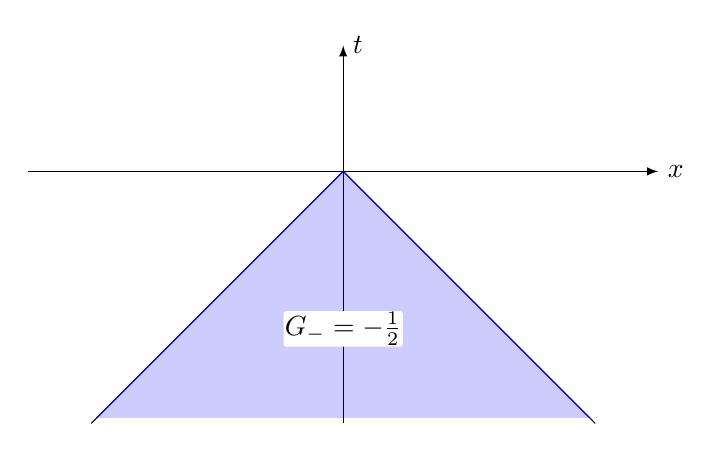
\begin{tikzpicture}[scale=0.8][>=latex]
	\coordinate (Origin)   at (0,0);
	\coordinate (XAxisMin) at (-5,0);
	\coordinate (XAxisMax) at (5,0);
	\coordinate (YAxisMin) at (0,-4);
	\coordinate (YAxisMax) at (0,2);
	\draw [thin,-latex] (XAxisMin) -- (XAxisMax) node[right] {$x$};% Draw x axis
	\draw [thin,-latex] (YAxisMin) -- (YAxisMax) node[right] {$t$};% Draw y axis
	
	%\clip (-5,-5) rectangle (10cm,10cm); % Clips the picture...
	
	\draw[thin] (0,0) -- (4,-4);
	\draw[thin] (0,0) -- (-4,-4);
	\begin{scope}
	\clip (-4,0) -- (4,0) -- (4,-3.9)-- (-4,-3.9) --cycle;
	\draw [thin, color=blue, fill=blue, fill opacity=0.2] (0,0) -- (4,-4) -- (-4,-4) --cycle ;
	\end{scope}
	\node[fill=white,rounded corners=1pt,inner sep=0.5pt] at (0,-2.5) {$G_-=-\frac{1}{2}$};
	
	
	
	
	
	
	\end{tikzpicture}

	\caption{The support of $G_-$ in 1+1 dimensional case.}
		\label{fig:1Dadvanced}
\end{figure}



From \textsc{Figure}s (\ref{fig:1Dretarded}) and (\ref{fig:1Dadvanced}) one can infer that the fundamental solutions are supported respectively on $J_+(0)$ and $J_-(0)$.

\subsection*{Dimension $n=1+2$ - wave on a surface}
The integral is two dimensional:
\[	G_{(2)}^{+}(t,\mf{x})=\frac{\Theta( t)}{(2\pi)^{2}}\lim_{\epsilon\to 0^+}\int_{\mR^{2}}\dd\mathbf{k}\,e^{i\mathbf{k}\cdot\mathbf{x}}\, \frac{\sin|\mathbf{k}|t}{|\mathbf{k}|}e^{-\epsilon|\mf{k}| t}.		\]
To evaluate it we switch to polar coordinates $\mf{k}=(k\cos\varphi,k\sin\varphi)$. With the integral measure
\[	\dd \mf{k}=k\, \dd k\,\dd\varphi	,	\]
the integral becomes ($x:=|\mf{x}|$)
\[	\int_{0}^{2\pi}\dd\varphi\int_{0}^{+\infty}\dd k\,e^{ik x\cos\varphi}	\sin k t\,e^{-\epsilon k t}.	\]
It holds that 
\[	\int_{0}^{\infty}\dd k\,e^{ik (y+i\epsilon)}	\sin k t=\frac{1}{2i}\left[\int_{0}^{+\infty}e^{ik (y+i\epsilon +t)}\,\dd k+\int_{0}^{+\infty}e^{i k (y+i\epsilon-t)}\,\dd k\right]=\] \[=\frac{1}{2}\left[I_\epsilon(y+t)+I_\epsilon(y-t)\right],		\]
where we set $\ds I_\epsilon(y):=\frac{1}{i}\int_{0}^{+\infty}e^{i k (y+i\epsilon)}\,\dd k$. Since
\[	I_\epsilon(y)= \frac{1}{i}\int_{0}^{+\infty}e^{i k (y+i\epsilon)}\,\dd k=\frac{1}{y+i\epsilon},	\]
the integral which needs to be evaluated is
\[	\frac{1}{2}\int_{0}^{2\pi}\left[\frac{1}{x\cos\varphi+t+i\epsilon}+\frac{1}{x\cos\varphi-t+i\epsilon}\right]\,\dd\varphi.	\]
Such integral has a counterpart over a unit circle in the complex plane with the substitutions $\dd\varphi=-i\dd z/z$ and $\cos\varphi=(z+z^{-1})/2$. Hence, using Cauchy residue theorem
\[	\int_{0}^{2\pi}\frac{1}{x\cos\varphi\pm t+i\epsilon}\,\dd\varphi=-2i\oint\frac{\dd z}{xz^2+2(\pm t+i\epsilon)+x}	=\frac{2\pi}{\sqrt{(t\mp i\epsilon)^2-x^2}}.	\]
Putting everything together in the weak limit $\epsilon\to 0$ it holds
\begin{equation}
G_{(2)}^{+}(t,\mf{x})=\frac{\Theta( t)}{2\pi}\frac{\Theta(t^2-|\mf{x}|^2)}{\sqrt{t^2-|\mf{x}|^2}}=\frac{\Theta( t)}{2\pi}\frac{\Theta(\gamma(x))}{\sqrt{\gamma(x)}},
\label{eq:green2d}
\end{equation}
where $\Theta(t^2-|\mf{x}|^2)$ stems from Proposition \ref{prop:spacelike}. As a by-product, $\supp (G_\pm)\subseteq J_{\pm}(0)$.
\begin{figure}[h]
	\centering
	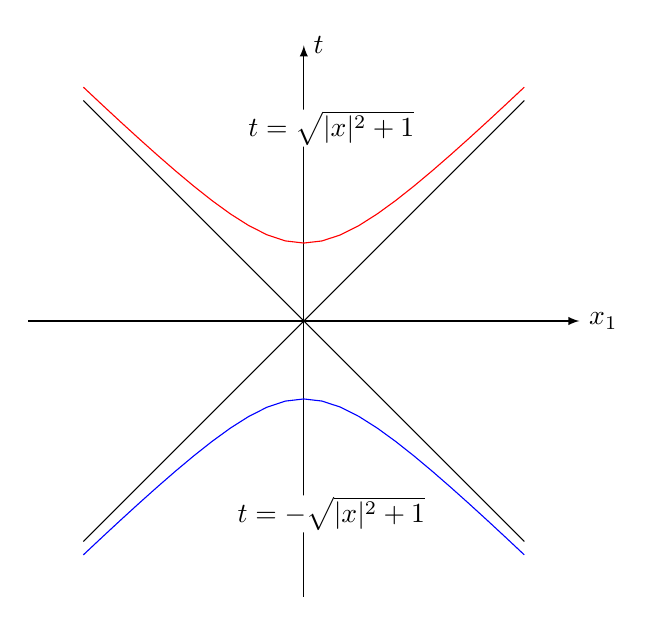
\begin{tikzpicture}[scale=0.7][>=latex]
	\coordinate (Origin)   at (0,0);
	\coordinate (XAxisMin) at (-5,0);
	\coordinate (XAxisMax) at (5,0);
	\coordinate (YAxisMin) at (0,-5);
	\coordinate (YAxisMax) at (0,5);
	\draw [thin,-latex] (XAxisMin) -- (XAxisMax) node[right] {$x_1$};% Draw x axis
	\draw [thin,-latex] (YAxisMin) -- (YAxisMax) node[right] {$t$};% Draw y axis
	%\draw [thin,-latex] (1.5,0.75) -- (-3,-1.5) node[left] {$x_2$};% Draw x axis
	
	%\clip (-5,-5) rectangle (10cm,10cm); % Clips the picture...
	
	\draw[thin] (0,0) -- (4,4);
	\draw[thin] (0,0) -- (-4,4);
	
	\draw[red] plot[domain=-4:4] (\x,{sqrt(\x* \x+2)});
	\node[fill=white,rounded corners=1pt,inner sep=0.5pt] at (0.5,3.5) {$t=\sqrt{|\mf{x}|^2+1}$};
	
	\draw[thin] (0,0) -- (4,-4);
	\draw[thin] (0,0) -- (-4,-4);
	
	\draw[blue] plot[domain=-4:4] (\x,{-sqrt(\x* \x+2)});
	\node[fill=white,rounded corners=1pt,inner sep=0.5pt] at (0.5,-3.5) {$t=-\sqrt{|\mf{x}|^2+1}$};
	
	
	
	
	
	
	\end{tikzpicture}
	\label{fig:2Dretarded}
	\caption{The level set $G_\pm(\mf{x},t)=1$ in the 1+2 dimensional case, plotted for one spatial axis.}
	
\end{figure}


\subsection*{Dimension $n=1+3$ - spherical wave}
The three-dimensional integral is
\[	G_{(3)}^{+}(t,\mf{x})=\frac{\Theta( t)}{(2\pi)^{3}}\lim_{\epsilon\to 0^+}\int_{\mR^{3}}\dd\mathbf{k}\,e^{i\mathbf{k}\cdot\mathbf{x}}\, \frac{\sin|\mathbf{k}|t}{|\mathbf{k}|}e^{-\epsilon|\mf{k}|t}.	\]

Again, we make a change of coordinate, switching to the spherical ones: $\mf{k}=(k\sin\theta\cos\varphi,k\sin\theta\sin\varphi,k\cos\theta)$. The integral measure reads
\[	\dd\mf{k}=k^2\sin\theta\,\dd k\,\dd\theta\,\dd\varphi		\]
and the integral to calculate is ($x:=|\mf{x}|$)
\[	\int_{0}^{2\pi}\dd\varphi\,\int_{0}^{+\infty}\dd k\,k\sin kt\int_{-1}^{1}	e^{ikx\cos\theta}\dd(\cos\theta)=\frac{4\pi}{x+i\epsilon}\int_{0}^{+\infty}\sin kt\sin k(x+i\epsilon)\,\dd k.	\]
Hence we can write using the exponential function
\[	\sin kt\sin kx=\frac{1}{4}\left\{\left[e^{ik(x+i\epsilon-t)}+e^{-ik(x+i\epsilon-t)}\right]-\left[e^{ik(x+i\epsilon+t)}+e^{-ik(x+i\epsilon+t)}\right]\right\},	\]
and with the change of variables $k\leftrightarrow-k$ it holds
\[	\frac{4\pi}{x}\int_{0}^{+\infty}\sin kt\sin kx\,\dd k=\frac{2\pi^2}{x}\frac{1}{2\pi}\int_{-\infty}^{+\infty}e^{ik(x+i\epsilon-t)}-e^{ik(x+i\epsilon+t)}\,\dd k\mathop{\longrightarrow}_{\epsilon\to 0^+}	\]
\[	\longrightarrow\frac{2\pi^2}{x}\left[\delta(t-x)-\delta(t+x)\right].		\]
To find the correct retarded and advanced fundamental solutions we notice that the second term, $\delta(t+x)$, vanishes for $G_+$ because $x>0$ and $t>0$. Conversely the first term $\delta(t-x)$ vanishes when computing $G_-$. In view of these considerations, the general formula for the $1+3$-case becomes
\begin{equation}
G_{(3)}^{+}(t,\mf{x})=\frac{\Theta( t)}{4\pi}\frac{\delta(t- |\mf{x}|)}{|\mf{x}|}.
\label{eq:green3d}
\end{equation}
One can verify that $G_{(3)}^{\pm}$ vanish outside the support of the delta distribution. Hence they are supported respectively on the upper and on the lower light cones $C_+(0)$ and $C_-(0)$. This is a particularity of the odd spatial dimensions, as we shall prove in the next section. This feature is known as the \textbf{Huygens' principle}. It states that in general, we have for spatial dimensions $d\neq 1$
\[	\supp\, G_{(d)}^{\pm}= J_{\pm}(0)\quad\text{for } d\text{ even},		\]
\[	\supp\, G_{(d)}^{\pm}= C_{\pm}(0)\quad\text{for } d\text{ odd.}		\]
Physically, we can see $\delta_0$ as a point source at $0$ of a signal that propagates with constant speed. Inside the future light cone the solution is zero, so if $d$ is even, the wave propagates strictly on the cone. In case $d$ is odd,
the signal of a point source propagates also inside the light cone. For an observer, the wave is noticeable not only at a single moment but still after the signal has arrived. An example of such
waves are the $2$-dimensional ones like water waves. For more on Huygens' principle, see [\citealp{gunther}] and [\citealp[Ch. 5]{jonsson}].








\begin{figure}[h]
	\centering
	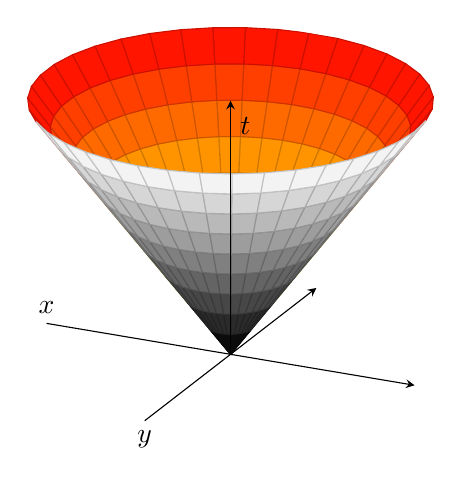
\begin{tikzpicture}
	\pgfplotsset{ticks=none}
	\begin{axis}[
	axis lines=center,
	axis on top,
	xlabel={$x$}, ylabel={$y$}, zlabel={$t$},
	domain=0:1,
	y domain=0:2*pi,
	%domain=-1:1,
	%y domain=-1:1,
	xmin=-1.5, xmax=1.5,
	ymin=-1.5, ymax=1.5, zmin=0.0,
	every axis x label/.style={at={(rel axis cs:0,0.5,0)},anchor=south},
	every axis y label/.style={at={(rel axis cs:0.5,0,0)},anchor=north},
	every axis z label/.style={at={(rel axis cs:0.5,0.5,0.9)},anchor=west},
	mesh/interior colormap name=hot,
	colormap/blackwhite, 
	%samples=40,
	%samples y=60,
	samples=10,
	samples y=40,
	z buffer=sort,
	]
	\addplot3 [surf, shader=faceted] ({(1.5*x*cos(deg(y))},{1.5*x*sin(deg(y))},{x});
	%\addplot3 [surf, shader=faceted] {sqrt(10*x*x+10*y*y+0.3)};
	\end{axis}
	\end{tikzpicture}
		\label{fig:3Dretarded}
	\caption{The support of $G_+$ in 1+3 dimensional case, i.e. the upper light cone $C_+(0)$, plotted for two spatial axis.}
\end{figure}


\noindent \large\textbf{The method of \emph{descent}}\footnote{see [\citealp[Ch. 6]{fried1}] and [\citealp[Ch. 5]{jonsson}].
}\\

	\noindent \normalsize The lower dimensional advanced and retarded distributions can be directly deduced from the $d=3$ case as we shall see. In general if we know the explicit solution to the $d$-dimensional case we can find the $d-1$-dimensional counterpart with the formula
	\[	G_{(d-1)}^{\pm}(t,x_1,\dots,x_{d-1})=\int_{-\infty}^{\infty}G_{(d)}^{\pm}(t,x_1,\dots,x_d)\,\dd x_{d}.	\]
	This technique is called \emph{method of descent}.
	The last assertion can be proven taking the fundamental solution equation
	\[\Box_d\, G_{(d)}(t,x_1,\dots,x_d)=\delta(t)\delta(x_1)\cdots\delta(x_d),\]
	where $\Box_d$ stands for $(\partial_t^2-\partial_1^2-\cdots-\partial_{d}^2)$. Integrating $G_{(d)}$ on the last variable against a test-function $\varphi\in\mD(\mR)$:
	\[	\int \Box_d\, G_{(d)}\,\varphi\,\dd x_d=	 \Box_{(d-1)}\int G_{(d)}\,\varphi\,\dd x_d-\int \partial_d^2 G_{(d)}\,\varphi\,\dd x_d=\] \[=\delta(t)\delta(x_1)\cdots\delta(x_{d-1})\int\delta(x_d)\varphi\,\dd x_d.	\]
	By letting the test-function become a sequence of cut-off functions covering the real axis, the formula
	\[	\Box_{(d-1)}\int G_{(d)}\,\dd x_d=\delta(t)\delta(x_1)\cdots\delta(x_{d-1})		\] is proven.\\
	To calculate the $d=2$ fundamental solution from the $d=3$ case, according to (\ref{eq:green3d}) and using equation (\ref{eq:delta1}) we can write for the retarded fundamental solution
	\[ \Theta(t)\frac{\delta(t-|\mf{x}|)}{2|x|}=\Theta(t)\delta(t^2-|\mf{x}|^2)=\Theta(t)\delta(t^2-x_1^2-x_2^2-x_3^2)=\] \[=\Theta(t)\Theta(t^2-x_1^2-x_2^2)\frac{\delta(x_3-\sqrt{t^2-x_1^2-x_2^2})+\delta(x_3+\sqrt{t^2-x_1^2-x_2^2})}{2\sqrt{t^2-x_1^2-x_2^2}},	\]
	where we insert the Heaviside step function to take into account Proposition \ref{prop:spacelike}. Hence, integrating over the third variable yields
	\[	G_{(2)}^{+}(t,x_1,x_2)=\frac{\Theta(t)}{2\pi}\frac{\Theta(t^2-x_1^2-x_2^2)}{\sqrt{t^2-x_1^2-x_2^2}}	,	\]
	which is identical to equation (\ref{eq:green2d}) as we expected. Similarly, the expression for the case $d=1$ can be derived again.\\
	
	If we now apply to the general expression for $G_{(d)}$ the Fourier transform in the last variable, similarly we obtain
	\[	\int_{-\infty}^{+\infty}\partial_d^2 G_{(d)}(t,x_1,\dots,x_d)e^{-im x_d}\,\dd x_d=\] \[=-m^2\int_{-\infty}^{+\infty} G_{(d)}(t,x_1,\dots,x_d)e^{-im x_d}\,\dd x_d=:-m^2\hat{G}_{d-1}(t,x_1,\dots,x_{d-1},m).	\]
	Hence, the Fourier transform on the last variable $\hat{G}_{d-1}(t,x_1,\dots,x_{d-1},m)$ is, for a fixed $m\in\mR$, a fundamental solution for the $d-1$ dimensional \textbf{Klein-Gordon} operator
	\[	\Box+m^2,	\]
	that describes the motion of spinless particles with mass $m$.

\section{The Riesz distributions}
\label{sec:riesz}

To discuss explicit and useful formulas for the fundamental solution in the general $n$-dimensional case, the approach we adopted in the last section is not very effective. We outline a method devised by M. Riesz in the first half of the 20th century in order to find solutions to a certain class of differential equations. We will follow [\citealp{ginoux}] and [\citealp[Ch. 1.3]{bar2}].
\begin{definition}
	For $\alpha\in\mC$ with $\Re\alpha>n$ let $R_\pm(\alpha)$ be the complex-valued continuous functions defined for any $x\in\mathbb{M}^n$ by
	\begin{equation}
		R_\pm(\alpha)(x):=\begin{cases}
		C(\alpha,n)\gamma(x)^{\frac{\alpha-n}{2}}\quad &\text{if }x\in J_{\pm}(0)\\
		0\qquad &\text{otherwise},\\
		\end{cases}
	\end{equation}
	where $\gamma$ is defined in Definition \ref{defn:gamma},
	\[	C(\alpha,n):=\frac{2^{1-\alpha}\pi^{\frac{2-n}{n}}}{\Gamma(\frac\alpha{2})\Gamma(\frac{\alpha-n}{2}+1)},		\]
	and $z\mapsto \Gamma(z)$ is the Gamma function.
	\label{defn:Rieszmink}
\end{definition}
\begin{rem}
	The functions $R_\pm(\alpha)$ are continuous because $\gamma=-\langle\cdot,\cdot\rangle_0$ vanishes on the boundary of $J_{\pm}(0)$ and the exponent $(\alpha-n)/2$ is assumed to have positive real part. If we increase the real part of the exponent then higher derivatives of the function vanishes at the boundary and the functions become more regular. As a matter of facts $R_\pm(\alpha)\in C^k(\mathbb{M}^n)$ whenever $\Re\alpha>n+2k$.
	\label{rem:regRiesz}
\end{rem}

\noindent Now we discuss the first properties of $R_\pm(\alpha)$.
\begin{prop}
	For all $\alpha\in\mC$ with $\Re\alpha>n$ it holds
	\begin{enumerate}
		\item[(1)] $\gamma\, R_\pm(\alpha) = \alpha(\alpha-n+2) R_\pm(\alpha+2);$
		\item[(2)] $(\grad \gamma)\, R_\pm(\alpha) = 2\alpha \grad R_\pm(\alpha+2);$
		\item[(3)] $\Box R_\pm(\alpha+2)  = R_\pm(\alpha)$.
	\end{enumerate}
	Moreover, the map
\begin{equation*}
\begin{aligned}
\mathds{X}_n &\to\mD'(\mathbb{M}^n)\\
\alpha &\mapsto R_\pm(\alpha) 
\end{aligned}
\end{equation*}
	(where $\mathds{X}_n:=\{\alpha\in\mC\,|\,\Re\alpha>n\}$) extends uniquely the whole complex plain as a holomorphic family of distributions, i.e. for each test-function $\varphi\in\mD(\mathbb{M}^n)$, the function $\alpha\mapsto (R_\pm(\alpha),\varphi)$ is holomorphic.
	\label{prop:firstRiesz}
\end{prop}
\Proof To prove (1), we evaluate $\gamma\,R_\pm(\alpha)$ inside $J_\pm(0)$, because both sides of the equation vanish outside. By definition one has
\[	\gamma\, R_\pm(\alpha) =	C(\alpha,n)\gamma(x)^{\frac{\alpha+2-n}{2}}	=\frac{C(\alpha,n)}{C(\alpha+2,n)}R_\pm(\alpha+2),	\]
and, in virtue of the fact that $z\Gamma(z-1)=\Gamma(z)$,
\[\frac{C(\alpha,n)}{C(\alpha+2,n)}=\frac{2^{1-\alpha}\pi^{\frac{2-n}{n}}}{(\frac{\alpha}{2}-1)!(\frac{\alpha-n}{2})!}\frac{(\frac{\alpha+2}{2}-1)!(\frac{\alpha+2-n}{2})!}{2^{1-\alpha-2}\pi^{\frac{2-n}{n}}}= \]
\[	=4\frac{\alpha}{2}\frac{\alpha+2-n}{2}=\alpha(\alpha-n+2).		\]
For the second identity we evaluate $\partial_i\gamma\cdot R_\pm(\alpha)$. In view of Remark \ref{rem:regRiesz}, $R_\pm(\alpha+2)\in C^1(\mathbb{M}^n)$ For any $\varphi$ integrating by parts yields:
\[	\begin{aligned}
\partial_i\gamma\cdot 	(R_\pm(\alpha),\varphi)&=C(\alpha,n)\int_{J_\pm}\gamma(x)^{\frac{\alpha-n}{2}}\partial_i\gamma(x)\varphi(x)\,\dd x\\
&=\frac{2C(\alpha,n)}{\alpha+2-n}\int_{J_\pm}\partial_i(\gamma(x))^{\frac{\alpha-n+2}{2}}\varphi(x)\,\dd x\\
&=-2C(\alpha+2,n)\int_{J_\pm}\gamma(x)^{\frac{\alpha-n+2}{2}}\partial_i\varphi(x)\,\dd x\\
&=-2\alpha(R_\pm(\alpha+2),\partial_i\varphi)\\
&=2\alpha(\partial_iR_\pm(\alpha),\varphi).
\end{aligned}	\]
To prove the third formula, from (2) we have
\[	\begin{aligned}
\partial_i^2R_\pm(\alpha+2)&=\partial_i\left(\frac{1}{2\alpha}\partial_i\gamma\cdot R_\pm(\alpha)\right)\\
&=\frac{1}{2\alpha}\partial_i^2\gamma\cdot R_\pm(\alpha)+\frac{1}{4\alpha(\alpha-2)}(\partial_i\gamma)^2\frac{(\alpha-2)(\alpha-n)}{\gamma}\cdot R_\pm(\alpha)\\
&=\left(\frac{1}{2\alpha}\partial_i^2\gamma+\frac{\alpha-n}{4\alpha}\cdot\frac{(\partial_i\gamma)^2}{\gamma}\right)\cdot R_\pm(\alpha).
\end{aligned}			\]
Applying $\Box$ we find
\[	\Box R_\pm(\alpha+2)=\left(\frac{n}{\alpha}+\frac{\alpha-n}{4\alpha}\cdot\frac{4\gamma}{\gamma}\right)R_\pm(\alpha)=R_\pm(\alpha),		\]
as claimed.\\
The last identity allows us to extend $R_\pm(\alpha)$ for every $\alpha\in\mC$.
For $\Re\alpha>n-2$ we set
\[	\widetilde{R}_\pm(\alpha):=\Box R_\pm(\alpha+2),		\]
and the extension is holomorphic on $\mathds{X}_{n-2}$. Now, proceeding by induction over $n$ one can extend the function over the whole complex plane.\endproof

\begin{figure}
\centering
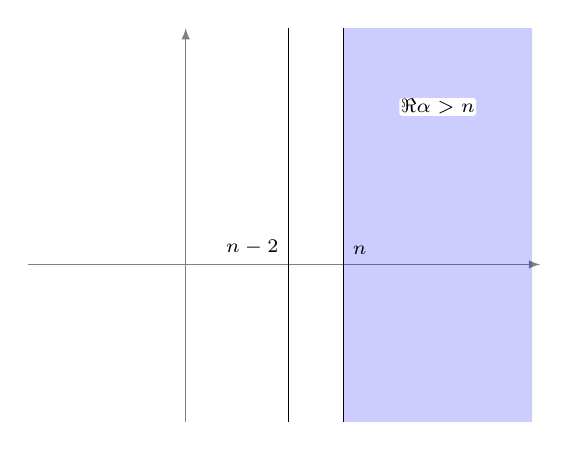
\begin{tikzpicture}
\tikzstyle{every node}=[font=\scriptsize]
\coordinate (Origin)   at (0,0);
\coordinate (XAxisMin) at (-2,0);
\coordinate (XAxisMax) at (4.5,0);
\coordinate (YAxisMin) at (0,-2);
\coordinate (YAxisMax) at (0,3);
\draw [thin, gray,-latex] (XAxisMin) -- (XAxisMax) ;% Draw x axis
\draw [thin, gray,-latex] (YAxisMin) -- (YAxisMax) ;% Draw y axis
\draw (1.3,-2)--(1.3,3);
\node[above left] at (1.3,0) {$n-2$};
\begin{scope}
\clip  (2,-2) -- (2,3) -- (4.4,3) -- (4.4,-2) -- cycle;
\draw [thin, color=blue, fill=blue, fill opacity=0.2] (2,-2.1) -- (2,3.1) -- (5,3.1) -- (5,-2.1) -- cycle;
\end{scope}
\draw (2,-2) -- (2,3);
\node[above right] at (2,0) {$n$};
\node[fill=white,rounded corners=1pt,inner sep=0.5pt] at (3.2,2) {$\Re\alpha>n$};
\end{tikzpicture}
\caption{Iterative extension of $R_\pm(\alpha)$ on $\mC$.}

\end{figure}


\begin{definition}
	The distributions $R_+(\alpha)$ and $R_-(\alpha)$ defined in the last proposition are called  respectively the \textbf{retarded} and \textbf{advanced} Riesz distributions for the parameter $\alpha\in\mC$.
\end{definition}


\noindent The Riesz distributions do not have an immediate explicit formula, but next lemma shows a more comfortable way to evaluate them when the test-function has a particular form. For the proof of this lemma, we remind to [\citealp[Lem 1.3.30]{bar2}].
\begin{lem}
	Denote $x=(t,\mf{x})$, with $\mf{x}\in\mR^{n-1}$. Let $f\in\mD(\mR)$ and let $\psi\in\mD(\mR^{n-1})$ be such that $\varphi(x):=f(t)\psi(\mf{x})\in\mD(\mathbb{M}^n)$ and $\varphi(x)=f(t)$ on $J_+(0)$. If $\Re\alpha>1$ it holds
	\begin{equation*}
		(R_\pm(\alpha),\varphi)=\frac{1}{(\alpha-1)!}\int_{0}^{+\infty}t^{\alpha-1}f(t)\,\dd t.
	\end{equation*}
\label{lem:Rieszevaluate}
\end{lem}
\noindent To link Riesz distributions to fundamental solutions the following facts are noteworthy.

\begin{prop}
	The Riesz distributions satisfy
	\begin{enumerate}
		\item[(1)] for any $\alpha\in\mC$, $\supp\,R_\pm(\alpha)\subset J_\pm(0)$
		\item[(2)] $R_\pm(0)=\delta_0$
		\item[(3)] $\Box R_\pm(2)=\delta_0$, in particular $R_+(2)$  and $R_-(2)$ are respectively a \textbf{retarded} and an \textbf{advanced} fundamental solution for $\Box$ at $0$.
	\end{enumerate}
\label{prop:secondRiesz}
\end{prop}
\Proof The first assertion descends from the definition of Riesz distributions.\\
To prove (2) fix $K\subset\mathbb{M}^n$ compact subset. Let $\sigma_K\in\mD(\mathbb{M}^n)$ such that $\sigma_K|_K=1$. For any $\varphi\in\mD(\mathbb{M}^n)$ with $\supp\,\varphi\subset K$ one finds suitable smooth functions $\varphi_j$ such that
\[\varphi(x)=\varphi(0)+\sum_{j=1}^{n}x^j\varphi_j(x),	\]

then it holds
\[	\begin{aligned}
(R_\pm(0),\varphi)&=(R_\pm(0),\sigma_K\varphi)\\&=\left(R_\pm(0),\varphi(0)+\sum_{j=1}^{n}x^j\varphi_j(x)\right)\\
&=\varphi(0)\overbrace{(R_\pm(0),\sigma_K)}^{=:c_K}+\sum_{j=1}^{n}\left(\overbrace{x^jR_\pm(0)}^{=0},\sigma_K\varphi_j\right)\\
&=c_K\varphi(0),
\end{aligned}			\]
where $x^jR_\pm(0)$ vanishes because of Equation (1) in Proposition \ref{prop:firstRiesz} one can show that $c_K$ does not depend on the choice of $K$ since for $K'\supset K$ and $\supp\,\varphi \subset K\subset K'$, $$c_K' \varphi (0) = (R_+ (0),\varphi) = c_K \varphi (0).$$
It descends $c_K = c_K' =: c$.  To show $c=1$, concentrating on the case of a retarded distribution, using test-functions as in Lemma \ref{lem:Rieszevaluate}, 
\[	\begin{aligned}
c\cdot\varphi(0)&=\left(R_+(0),\varphi\right)\\
&=\left(\Box R_+(2),\varphi\right)=\left( R_+(2),\Box\varphi\right)\\
&=\int_{0}^{+\infty}t\,f''(t)\,\dd t=-\int_{0}^{+\infty}f'(t)\,\dd t\\
&=f(0)=\varphi(0),
\end{aligned}		\]
which concludes the proof.\\
The third assertion is obtained considering (1) and making use of Equation (3) in Proposition \ref{prop:firstRiesz}.\endproof
\begin{rem}
	We will prove in Chapter \ref{chapter3} that the retarded and the advanced fundamental solutions are \textbf{unique}. Hence, we have
	\[	G_\pm=R_\pm(2).			\]
\end{rem}
\begin{rem}
	As one expects, if $\alpha\in\mR$, then $(R_\pm(\alpha),\varphi)$ is real for any $\varphi\in\mD(\mathbb{M}^n,\mR)$ i.e. $R_\pm(\alpha)$ is a real-valued distribution.
\end{rem}

\noindent We are now ready to prove \textbf{Huygens' principle}, that we already mentioned before. One can restate it as follows.

\begin{theorem}[\textbf{Huygens' principle}]
	If $n\geq 4$ is even, $\supp\,G_\pm= C_\pm(0)$.
	If $n\geq 3$ is odd, $\supp\,G_\pm= J_\pm(0)$.
	\label{th:Huygens}
\end{theorem}
\noindent To prove it we work with Riesz distributions and we need the following lemma\footnote{see [\citealp[Prop. 1.3.31]{bar2}]}.

\begin{lem}
	The following holds:
	\begin{enumerate}
	\item[(1)] for every $\alpha\in\mC\setminus(\{0,-2,-4,\dots\}\cup\{n-2,n-4,\dots\})$ we have $\supp\,R_\pm(\alpha)=J_\pm(0);$
	\item[(2)] for $n\geq 3$ and $\alpha=n-2,n-4,\dots,1$ if $n$ is odd or $\alpha=n-2,n-4,\dots,2$ if $n$ is even, we have
	$ \supp\,R_\pm(\alpha)=C_\pm(0). $
	\end{enumerate}
\end{lem}

\noindent \textbf{Proof of Theorem \ref{th:Huygens}.} The fundamental solutions are $G^\pm=R_\pm(2)$, so $\alpha=2$. Since $2=(n-2)+(4-n)$, if $n\geq 4$ and $n$ is even, $2\in\{n-2,n-4,\dots\}$; conversely, if $n$ is odd $2$ is not in $\{n-2,n-4,\dots,1\}$. So the theorem follows from the last lemma.\endproof


\section{General solution and Cauchy problem}
\label{sec:cauchymink}

We found the fundamental solution for the d'Alembert wave operator for the point $x_0=0$. To find the generic solution at a point $y\in\mathbb{M}^n$, as we have seen in Proposition \ref{prop:regularity}, it suffices to write
\[G_y^{+}(x)=T_yG_+=G_+(x-y).\]
Hence, to find the retarded solution $u_+(x)$ to the wave equation $\Box u=\psi$, where $\psi$ is a distribution, we simply evaluate the convolution
$G_+*\psi$. 
The general solution is obtained by adding the solutions of the homogeneous equation as in Formula \eqref{eq:homo}.\\

\noindent Now we discuss the uniqueness of the distributional solution and for its regularity we refer to Proposition \ref{prop:regularity}.\\
To begin, we shall prove the following\footnote{see [\citealp[Sec. 5.3]{jonsson}]}
\begin{theorem}
	Let $\psi\in\mD'(\mathbb{M}^n)$ such that $\psi(t,\mf{x})=0$ if $t<0$. Then $\psi$ and $G_+$ can be convoluted and $u_+=G_+*\psi$ is the unique solution to the wave equation with source $\psi$ such that $u_+(t,\mf{x})=0$ for $t<0$.
	
\end{theorem}
\Proof At fixed $x$, the distribution $G_+(x-y)\psi(y)$ has compact support in the variable $y$, so $G_+$ and $\psi$ can be convoluted. Since $\supp\, G_+\subset J_+(0)$, $u_+=0$ for $t<0$.\\
The solution is unique because if there were another $u$ solving the equation and satisfying the requested conditions, then $\phi:=u_+-u$ would be a solution to the homogeneous equation, i.e. $\Box \phi=0$, and $\phi$ could be convoluted with $G_+$:
\[	\phi=\phi*\delta=\phi*\Box\, G_+=\Box\,\phi*G_+=0,		\]
hence $u=u_+$.\endproof\\

\noindent Remaining in the Minkowski case, since $\mathbb{M}^n$ is a globally hyperbolic manifold, we can find smooth Cauchy hypersurfaces, where we can assign initial values.\\
Physically, it is clear why these can only be specified on a spacelike surface. A wave cannot travel from one point of the initial value surface to another and change the initial conditions.
\begin{definition}
	Let $S$ be a smooth Cauchy hypersurface of $\mathbb{M}^n$ with a timelike oriented unit normal vector field $n:S\to\mT\mathbb{M}^n$.\\ Given a triple $(\psi,u_0,u_1)\in\mD(\mathbb{M}^n)\oplus\mD(S)\oplus\mD(S)$, we call a \textbf{classical Cauchy problem} for $\Box$ on $S$ the system of equations
	\begin{equation}
	\begin{cases}
	\Box u=\psi\\
	\\
	u|_S=u_0\\
	\\
	\partial_n u|_S=u_1.
	\end{cases}
	\end{equation}
	In case the triple is taken in $\mD'(\mathbb{M}^n)\oplus\mD'(S)\oplus\mD'(S)$, i.e. the data are distributions, the problem is called \textbf{generalized Cauchy problem}.
\end{definition}

\noindent For simplicity, we concentrate on the case where $S$ is the hyperplane $$S_0:=\{(t,\mf{x})\in\mM\,|\, t=0\},$$ and $\partial_n=\partial_t$. The general case will be addressed later in Section \ref{sec:globalCauchy}, when we will discuss of Cauchy problem on manifolds. To solve the initial value problem, we start with a lemma

\begin{lem}
	Suppose $u$ is a solution for the Cauchy problem on $S_0$. If we set 
	\[	\tilde{u}(t,\mf{x}):=\begin{cases}
	u(t,\mf{x})\quad\text{if }& t>0\\
	0&\text{otherwise},
	\end{cases}			\]
	\[	\tilde{\psi}(t,\mf{x}):=\begin{cases}
	\psi(t,\mf{x})\quad\text{if }& t>0\\
	0&\text{otherwise},
	\end{cases}			\] it holds
	\begin{equation}
	\Box\, \tilde{u}(t,\mf{x})=\tilde{\psi}(t,\mf{x})+u_0(\mf{x})\delta'(t)+u_1(\mf{x})\delta(t).
	\end{equation}
\end{lem}
\Proof Let $\varphi\in\mD'(\mathbb{M}^n)$, then
\[(\Box\tilde{u},\varphi)=(\tilde{u},\Box\varphi)=\int_{0}^{\infty}\dd t\int u\,\Box\varphi\,\dd\mf{x}= \]
integrating by parts in the time variable
\[=\int_{0}^{\infty}\dd t\int \Box u\,\varphi\,\dd\mf{x}+\int \partial_t u(0,\mf{x})\,\varphi(0,\mf{x})-u(0,\mf{x})\,\partial_t \varphi(0,\mf{x})\,\dd\mf{x}=   \]
\[	=\int \tilde{\psi}+u_1\delta(t)+u_0\delta'(t)\,\dd t\,\dd\mf{x}. 			\]\endproof




\begin{theorem}[\footnote{see [\citealp[Th. 5.3.2]{jonsson}]}]
	If $u_\pm\in C^\infty(\mathbb{M}^n)$ solves the Cauchy problem on $S_0$ and $\supp\,u_\pm\subset J_\pm(K)$, where $K:=\supp\, u_0\cup\supp\,u_1\cup\supp\,\psi$, then it holds
	\begin{equation}
		u_\pm=G_\pm*(\psi+u_0\otimes\delta'+u_1\otimes\delta).
	\end{equation}
	\label{th:deltaprimo}
\end{theorem}

\noindent This leads to the following Corollary, that will be addressed in the general setting in Section \ref{sec:globalCauchy}.

\begin{cor}
	If $u\in C^\infty(\mathbb{M}^n)$ solves the Cauchy problem on $S_0$ with $Pu=0$ (i.e. $\psi=0$), then
	\[\supp\,u\subset J_+(K)\cup J_-(K),\]
	where $K:=\supp\,u_0\cup\supp\,u_1$, and a solution is given by
	\begin{equation}
u=G*(u_0\otimes\delta'+u_1\otimes\delta)
\end{equation}
	for all $\varphi\in\mD(\mathbb{M}^n)$, where $G=G_+-G_-$.
	\label{cor:homogeneousmink}
\end{cor}




\noindent Now follows the general result on $S_0$.
\begin{theorem}
	For each $(\psi,u_0,u_1)\in\mD(\mathbb{M}^n)\oplus\mD(S_0)\oplus\mD(S_0)$, there exists a unique solution $u$ to the Cauchy problem on $S_0$. Furthermore $\supp\,u\subset J_+(K)\cup J_-(K)$, where $K:=\supp\, u_0\cup\supp\,u_1\cup\supp\,\psi$.
\end{theorem}
\Proof We will only prove the existence. To build it with initial values $u_0,u_1$ we need the sum of a particular solution and the solution for the homogeneous equation.\\
We start by noting that a particular solution of $\Box\widetilde{\phi}=\psi$ induces initial values on $S_0$ given by $\widetilde{u}_0(\mf{x})=G_+*\psi(0,\mf{x})$ and $\widetilde{u}_1(\mf{x})=\partial_t G_+*\psi(0,\mf{x})$. Hence, for the homogeneous equation with initial values $u_0,u_1$, we apply Corollary \ref{cor:homogeneousmink} with initial values $u_0-\widetilde{u}_0$ and $u_1-\widetilde{u}_0$ and find $\widehat{\phi}$.\\
The general solution will be $\phi=\widehat{\phi}+\widetilde{\phi}$.\endproof\\





\noindent The solution, if we concentrate on the classical Cauchy problem, is smooth (Proposition \ref{prop:regularity}) and depends continuously on the initial data, hence the map that gives the solution $u$ can be seen as a \textbf{linear continuous operator}
\begin{equation*}
\begin{aligned}
\mD(\mathbb{M}^n)\oplus\mD(S)\oplus\mD(S)&\to C^{\infty}(\mathbb{M}^n)\\
(\psi,u_0,u_1)&\mapsto u.
\end{aligned}
\end{equation*}


